%Übersicht ist in getrennter Datei textdokumente-uebersicht.
\paragraph{Vertiefung}
Texdokumente und Textdateien bestehen aus einer Folge von Zeichen, die Wörter, Sätze und Absätze bilden. Auf Maschinenebene werden diese Zeichen durch Zahlenwerte gespeichert und die Zeichenkodierung beschreibt, welcher Zahlenwert für welches Zeichen steht. 

Wie ein Zeichen dargestellt wird, hängt von der verwendeten Schriftart, dem sogenannten Font ab, der einen Satz an Bildern für die verschiedenen Schriftzeichen bereitstellt.

Die Inhalte von Textdateien können durch die Verwendung einer Auszeichnungssprache strukturiert und beschrieben werden und somit auch eine maschinelle Verarbeitung ermöglichen.

\subparagraph{Zeichenkodierung und Zeichensatz} 
Zur korrekten Darstellung der Zeichen in einem Textdokument muss der Computer wissen, welche Zeichenkodierung (\emph{encoding}) verwendet wird. Auf Maschinenebene wird ein Zeichen als eine Folge von Nullen und Einsen, in Form von Bytes gespeichert, die wiederum bestimmte Zahlenwerte angeben. Diese Zahlenwerte können in Abhängigkeit der Zeichenkodierung unterschiedlich interpretiert werden.

Eine Zeichenkodierung kann abstrakt als eine Tabelle verstanden werden, in der einer bestimmten Zeichenmenge, dem Zeichensatz, Zahlenwerte zugeordnet werden. Beispielsweise hat der Buchstabe \emph{A} in dem \emph{American Standard Code for Information Interchange} (ASCII) den dezimalen Zahlenwert von \emph{65}. Der ASCII-Zeichensatz besteht aus insgesamt 128 Zeichen die jeweils mit einem Byte gespeichert werden. Er enthält keine diakritischen Zeichen, wie etwa \emph{ä}, oder gar andere Schriften, weshalb verschiedene Erweiterungen der ASCII-Kodierung entwickelt wurden, um insgesamt 256 verschiedene Zeichen zu kodieren. 

Beispiele für diese Erweiterungen sind ISO 8859-1 für lateinische Schriften oder ISO 8859-7 für das griechische Alphabet. In beiden Zeichenkodierungen hat das Zeichen \emph{A} jeweils den Wert \emph{65}. Jedoch stellt der Wert \emph{228} in ISO 8859-1 das Zeichen \emph{ä} und in ISO 8859-7 das Zeichen \emph{$\delta$} dar. Die Angabe der verwendeten Zeichenkodierung ist entscheidend dafür, ob auf dem Bildschirm \emph{ôå$\div$íç} oder \emph{$\tau\epsilon\chi\nu\eta$} dargestellt wird. %ôå÷íç

In der Vergangenheit war es besonders schwierig, wenn in einem Text gleichzeitig Umlaute und griechische Buchstaben verwendet werden sollten, da jede ASCII-Erweiterung jeweils nur insgesamt 256 Zeichen kodiert und einem Dokument nicht mehr als eine Zeichenkodierung zugewiesen werden kann. Deshalb wurde Unicode entwickelt.

Unicode ist ein Zeichensatz, in dem aktuell für 113.021 Zeichen aus 123 Schriftsystemen eindeutige Codepunkte (\emph{code points}) zugewiesen werden. Die Codepunkte werden mittels einer hexadezimalen Zahl und einem vorangestellten \emph{U+} dargestellt, wie beispielsweise \emph{U+00C4} für \emph{ä}. Zugleich stellt dieser Zeichensatz die Umsetzung von dem in ISO 10646 beschriebenen universellen Zeichensatz \emph{Universal Character Set} dar.

Um den Unicode-Zeichensatz in einem System anwenden zu können, wurden Zeichenkodierungen definiert, die unter dem Namen \emph{Unicode Transformation Format} (UTF) subsumiert werden. Zu den häufigsten gehören dabei UTF-8 und UTF-16, die im Web und in verschiedenen Betriebssystemen eine große Verbreitung gefunden haben. Der Unterschied besteht dabei in der Zahl der pro Zeichen verwendeten Bytes. Eine Besonderheit von UTF-8 besteht darin, dass die Bytedarstellungen der ersten 128 Zeichen denen der 128 Zeichen des ASCII-Zeichensatzes entspricht.

Das Unicode-Zeichen \emph{U+FEFF} gibt am Anfang des kodierten Dokumentes an, in welcher Reihenfolge die Bytes angeordnet sind. Diese Bytereihenfolge-Markierung (engl. \emph{byte order mark}) wird als \emph{BOM} abgekürzt und ist bei der Verwendung von UTF-16 und UTF-32 zwingend in der Datei erforderlich. Zusätzlich kann das BOM ein Hinweis auf die Verwendung von UTF-Kodierungen sein, jedoch wird von dessen Verwendung außer für UTF-16 und UTF-32 abgeraten.


\subparagraph{Schriftart}
Das optische Erscheinungsbild eines Textdokumentes hängt vorwiegend von den verwendeten Schriftarten (Fonts) ab. Es handelt sich dabei um die elektronische Form von Schriftarten, die für jedes Zeichen eine Raster- oder Vektorgrafik zur Verfügung stellt. 

Nicht auf jedem Rechner sind die gleichen Schriftarten installiert. Wenn ein Textdokument auf einem anderen System geöffnet wird, wo die Schriftarten nicht verfügbar sind, werden diese automatisch durch andere ersetzt. Das kann zu Inkonsistenzen der Dokumentdarstellung auf unterschiedlichen Systemen führen, weil beispielsweise Wörter, Sätze oder Absätze von einer Seite auf die nächste oder vorhergehende wandern, was für die Referenzierung von Inhalten problematisch ist.  

Daher muss für Dokumente, deren optischer Eindruck erhalten bleiben soll, zumindest der verwendete Font in den Metadaten angegeben werden. Wenn es das Format erlaubt, kann der Font auch in die Datei eingebettet werden, was im Praxisteil ab Seite \pageref{text-fontembedding} erläutert wird.


\subparagraph{Auszeichnungssprachen}\label{text-auszeichnungssprachen}
Der Inhalt von reinen Textdateien kann durch die Verwendung von Auszeichnungssprachen (\emph{Markup Languages}) näher beschrieben werden. Beispielsweise können verschiedene Gliederungsebenen mit Hilfe von bestimmten Auszeichnungselementen (auch \emph{Tags}) annotiert werden. Wie diese Tags aussehen und wie sie angewendet und kombiniert werden können, beschreibt eine Dokumentgrammatik. 

Abstrakt können Tags mit Etiketten verglichen werden, die einzelne Wörter, Wortgruppen oder ganze Textbereiche umschließen. Abbildung \ref{abb:Text-Tag} veranschaulicht, wie mit einem Tag die Zeichenkette "`\emph{24-28}"' als Größenangabe etikettiert wird. Das Tag besteht aus einem öffnenden Teil vor und einem schließendem Teil nach der fraglichen Zeichenkette, wobei das schließende Element zusätzlich durch einen Schrägstrich gekennzeichnet ist.

%Code-Block, der in das folgende Bild eingefügt wird
\newsavebox{\singleTag}
\begin{lrbox}{\singleTag}
\lstset{language=XML}
\begin{lstlisting}[mathescape]
<groesse>24-28</groesse>
\end{lstlisting}
\end{lrbox}

\begin{wrapfigure}{r}{0.4\textwidth}
%\begin{center}
	\usebox{\singleTag}
	\caption{Die Zeichenkette "`\emph{24-28}"' wird durch das Umschließen mit einem Tag als Größenangabe gekennzeichnet.}
%\end{center}
\label{abb:Text-Tag}
\end{wrapfigure}

Mit Hilfe von Auszeichnungssprachen wird das Aussehen eines Textdokumentes von dessen Struktur und Inhalt getrennt. Beispielsweise basieren Webseiten auf HTML-Dateien in denen Überschriften, Absätze, Links etc. mit Tags gekennzeichnet werden, die den Inhalt strukturieren. Wie dann beispielsweise die Überschriften formatiert werden, hängt von einer zusätzlichen Datei mit Formatierungsangaben ab, die austauschbar ist.

Die Grundlage vieler heute verwendeter Auszeichnungssprachen bildet die Standard Generalized Markup Language (SGML, Normierte Verallgemeinerte Auszeichnungssprache), die seit 1986 ein ISO-Standard (ISO 8879) ist. Die Regeln für die zu verwendenden Auszeichnungselemente und deren Kombinationsmöglichkeiten sind üblicherweise in einer externen Datei hinterlegt und werden zu Beginn der Datei in der Dokumenttypdeklaration angegeben. Bei SGML handelt es sich dabei um die sogenannte Dokumenttypdefinition (DTD).

Eine Anwendung von SGML ist die Hypertext Markup Language (HTML, Hypertext-Auszeichnungssprache), welche als Grundlage von Webseiten eine sehr große Verbreitung gefunden hat. HTML wird vom World Wide Web Consortium (W3C) und der Web Hypertext Application Technology Working Group (WHATWG) gepflegt und entwickelt. Die aktuellste Version ist HTML5.

Eine Teilmenge von SGML bildet die Extensible Markup Language (XML, Erweiterbare Auszeichnungssprache) und erlaubt im Gegensatz zu HTML die Definition von eigenen Auszeichnungselementen, um beliebige Strukturen annotieren zu können. De facto wurde SGML von der einfacher anwendbaren XML verdrängt. Auch XML wird vom W3C gepflegt und entwickelt. XML bildet die Grundlage von vielen weiteren Dateiformaten wie ODT, DOCX, SVG etc. Für XML-Dateien gibt es als Alternative zu einer DTD die Möglichkeit der Verwendung eines XML Schemas (XSD, XML Schema Definiton).

Auszeichnungssprachen kennzeichnen implizite Informationen, die nur für den menschlichen Leser verständlich sind, explizit. Dadurch wird ein Dokument maschinenlesbar und eine automatische Verarbeitung von semantisch annotierten Informationen in Texten möglich. Beispielsweise kann eine Münze mit Tags beschrieben werden, die das Material, das Gewicht, die Größe, den Avers und Revers kennzeichnen. So weiß auch ein Computerprogramm, welche Zeichenfolge in einer Datei sich auf das Material oder das Gewicht einer Münze bezieht.

Speziell für die Geistes"=, Sozial"= und die Sprachwissenschaften wird von der Text Encoding Initiative (TEI) ein auf XML basierendes Dokumentenformat entwickelt, das den Austausch von maschinenlesbaren Texten unterstützen und standardisieren soll. Die aktuelle Version ist P5.

%Code-Block, der in das folgende Bild eingefügt wird
\newsavebox{\muenze}
\begin{lrbox}{\muenze}
	\lstset{language=XML}
	\begin{lstlisting}[mathescape]
	<objekt typ="muenze">
	<material>Silber</material>
	<gewicht einheit="gramm">16,96</gewicht>
	<groesse einheit="mm">24-28</groesse>
	<avers>Kopf der Athena</avers>
	<revers>$A\Theta E$. Eule</revers>
	</objekt>
	\end{lstlisting}
\end{lrbox}

\begin{wrapfigure}{r}{0.59\textwidth}
	\begin{subfigure}{.585\textwidth}
		\centering
		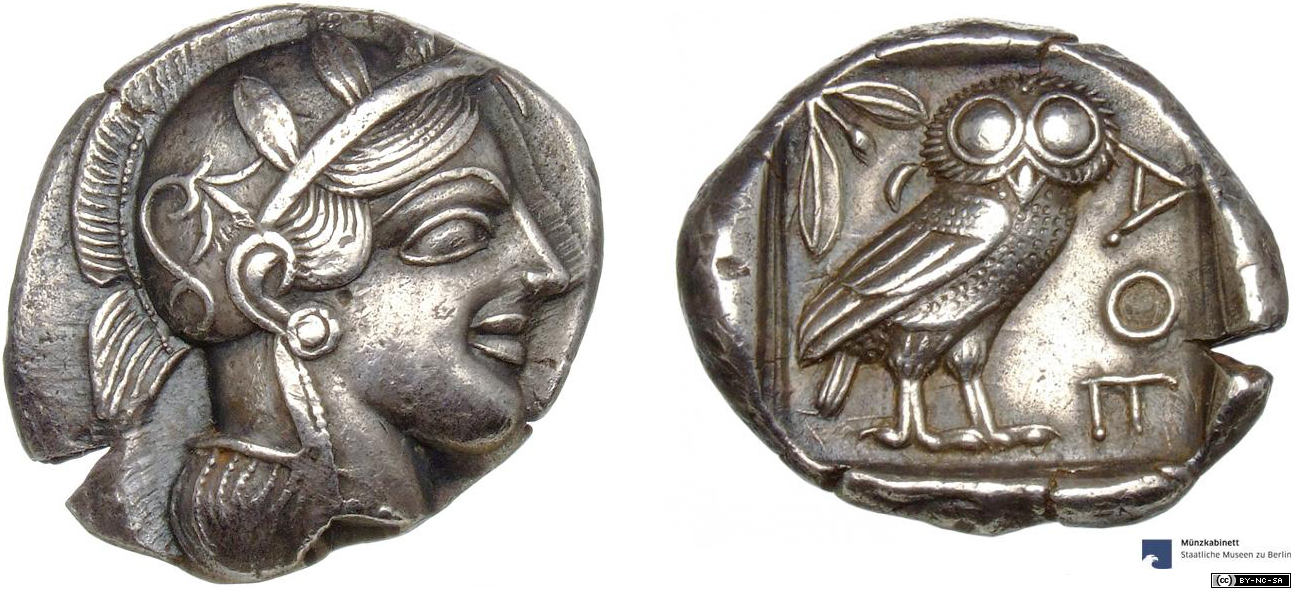
\includegraphics[width=\linewidth]{bilder/text_muenze}
	\end{subfigure}\linebreak
	\begin{subfigure}{.585\textwidth}
		\usebox{\muenze}
	\end{subfigure}
	\caption{Tetradrachme; Objektnummer \href{http://ww2.smb.museum/ikmk/object.php?id=18214973}{18214973} \href{http://ww2.smb.museum/ikmk/index.php}{Münzkabinett -- Staatliche Museen zu Berlin}, Lizenz: \href{http://creativecommons.org/licenses/by-nc-sa/3.0/de/}{CC-BY-NC-SA 3.0} mit einer Beschreibung in XML-Form. Das Material, das Gewicht, die Größe, der Avers und Revers sind mit Tags gekennzeichnet. Zusätzlich ist die Maßeinheit von Gewicht und Größe als Attribut angegeben.}
\end{wrapfigure}

Es gibt weitere Auszeichnungssprachen, die speziell die Darstellung der Dokumente beschreiben, also definieren, wie ein Dokument auf dem Bildschirm oder gedruckt aussehen soll. Beispiele hierfür sind das Textsatzsystem \TeX  mit dem Makropaket \LaTeX, PDF oder PostScript.

Es ist erforderlich, dass alle Dateien, die Auszeichnungssprachen verwenden, wohlgeformt und valide sind. Wohlgeformt meint das Einhalten der Regeln der jeweiligen Auszeichnungssprache. Die Validität bezieht sich auf die verwendete Grammatik und gilt insbesondere für SGML-, HTML- und XML-Dateien. Beispielsweise muss eine XML-Datei einen Verweis auf eine DTD oder ein XML Schema enthalten und auch die dadurch vorgegebene Struktur einhalten, um als valide zu gelten.


\paragraph{Praxis}
Dieser Abschnitt liefert Hinweise zum Umgang mit Textdokumenten und Textdateien in der Praxis. Es wird erläutert, was bei der Speicherung von Textdokumenten mit Formatierungsangaben zu beachten ist und wie Schriftarten eingebettet werden können. Speziell für Textdateien werden Texteditoren und das Einstellen der Zeichenkodierung thematisiert. Auch Hinweise zur Ergänzung und Extraktion von Metadaten werden gegeben. Für die Digitalisierung von Texten wurden die wichtigsten Informationen aus den DFG-Praxisregeln "`Digitalisierung"' zusammengefasst.

\subparagraph{Textdokumente mit Formatierungsangaben} Textdokumente mit Formatierungsangaben, wie verschiedene Schriftgrößen, Fett- oder Kursivschreibung, oder in welche zusätzlich Medien, wie Bilder, Tabellen oder Videos integriert sind, erfordern eine besondere Aufmerksamkeit bei der Speicherung. Das gilt insbesondere wenn bestimmte Formatierungen von Textelementen mit einer Bedeutung verbunden sind und die Authentizität des Erscheinungsbildes, also das Aussehen des Dokumentes, wichtig ist, denn dasselbe Dokument könnte auf verschiedenen Systemen unterschiedlich dargestellt werden.  

Für die Bearbeitung von Textdokumenten mit Formatierungsangaben und eingebetteten Medien gibt es dezidierte Textverarbeitungsprogramme, wie OpenOffice Writer, LibreOffice Writer oder Microsoft Word. OpenOffice und LibreOffice speichern Textdokumente standardmäßig im ODT-Format. Seit 2007 speichert Microsoft Word im DOCX-Format. Beide Formate sind offen dokumentiert, basieren auf XML und sind für die Langzeitarchivierung geeignet. In allen genannten Programmen ist die Zeichenkodierung bereits auf UTF-8 voreingestellt.

Eingebettete Bilder oder andere Medien sollten zusätzlich als separate Dateien in einem geeigneten Langzeitformat gespeichert werden. Dies stellt sicher, dass die Qualität der ursprünglichen Datei erhalten bleibt.

Die Darstellung von Textdokumenten kann auf verschiedenen Computern unterschiedlich ausfallen, was vor allem an unterschiedlichen Einstellungen liegt. Wenn bestimmte Schriftarten auf einem System fehlen, werden sie automatisch ersetzt, was ebenfalls zu unterschiedlichen Darstellungsweisen führt. Daher sollten nach Möglichkeit die verwendeten Schriftarten eingebettet werden, was im nächsten Unterabschnitt erläutert wird.

Eine stabile systemübergreifende Darstellung von Textdokumenten kann nur mittels Konvertierung in ein PDF-Dokument gewährleistet werden. Für die Langzeitspeicherung sollte PDF/A verwendet werden. Hinweise zum Erstellen von PDF- und PDF/A-Dokumenten sind im Praxisteil zu PDF-Dokumenten ab Seite \pageref{pdf-dokumenteErstellen} zu finden.

\begin{flushleft}
	OpenOffice Writer: \urllist{https://www.openoffice.org/}
	LibreOffice Writer: \urllist{http://www.libreoffice.org/}
\end{flushleft}


\subparagraph{Einbettung von Schriftarten}\label{text-fontembedding}
Da das optische Erscheinungsbild eines Textdokumentes unter anderem von den verwendeten Schriftarten abhängt, kann die Einbettung derselben ratsam sein. Dabei muss darauf geachtet werden, dass die Lizenzen für die verwendeten Fonts vorhanden sind.

Ab Version 4.1 können in LibreOffice die benutzten Fonts in das ODT-Format eingebettet werden. Dazu im Menü auf "`Datei > Eigenschaften"' gehen, in dem Dialog den Reiter "`Schriftart"' anwählen und dort den Haken bei "`Schriftarten ins Dokument einbetten"' setzen. Dieser Vorgang muss für neue oder andere Dokumente wiederholt werden. 

Auch in Microsoft Word ist diese Einstellung für das DOCX-Format möglich. Dazu auf "`Datei > Optionen"' gehen, in dem Dialog den Punkt "`Speichern"' auf der linken Seite auswählen und einen Haken bei "`Schriftarten in der Datei einbetten"' setzen. Diese Einstellung ist ebenfalls nur für das aktuelle Dokument gültig und muss bei anderen Dokumenten bei Bedarf wiederholt werden.

Werden Textdokumente als PDF exportiert, so werden die verwendeten Schriftarten automatisch eingebettet. Aktuell funktioniert die Einbettung von Fonts in andere Dateiformate als PDF nicht völlig fehlerfrei.


\subparagraph{Texteditoren und Editoren für Auszeichnungssprachen}
Für die Bearbeitung von Textdateien wie TXT, XML oder HTML sind einfache spezialisierte Texteditoren am besten geeignet. In den verschiedenen Betriebssystemen ist üblicherweise mindestens ein Texteditor vorinstalliert, wie beispielsweise \emph{Editor} oder \emph{Notepad} bei Microsoft Windows. Im Vergleich zu Textverarbeitungsprogrammen ist der Funktionsumfang bei Texteditoren deutlich kleiner, was bei reinen Textdateien aber kein Nachteil ist.

Gerade für den täglichen Umgang mit Textdateien empfiehlt sich die Verwendung von leistungsfähigen Editoren, die neben ausgefeilten Suchfunktionen auch Autovervollständigung oder für Auszeichnungssprachen Syntaxhervorhebung bieten. Für Mac OS X gibt es beispielsweise \href{http://www.barebones.com/products/textwrangler/}{TextWrangler} und für Windows \href{http://www.notepad-plus-plus.org/}{Notepad++} als kostenlose Angebote. Eine umfangreiche vergleichende Liste von Texteditoren ist auf \href{http://en.wikipedia.org/wiki/Comparison_of_text_editors}{Wikipedia} zu finden. 

Für den regelmäßigen Umgang mit einem bestimmten Format, wie etwa HTML oder XML, können weiter spezialisierte Editoren praktisch sein.

\begin{flushleft}
	Notepad++: \urllist{http://www.notepad-plus-plus.org/}
	TextWrangler: \urllist{http://www.barebones.com/products/textwrangler/}
	Vergleich von Texteditoren auf Wikipedia: \urllist{http://en.wikipedia.org/wiki/Comparison_of_text_editors}
\end{flushleft}


\subparagraph{Einstellen der Zeichenkodierung}\label{text-encodingEinstellen}
Wenn keine besonderen Anforderungen dagegen sprechen, sollte Unicode für die Zeichenkodierung verwendet werden. Dabei sollte UTF-8 ohne BOM bevorzugt werden. 

In modernen Textverarbeitungsprogrammen, die DOCX oder ODT speichern, ist dies für die genannten Formate voreingestellt und muss nicht explizit angepasst werden.

Bei der Bearbeitung von Textdateien mit Texteditoren muss auf die richtigen Einstellungen und Speicheroptionen geachtet werden. Insbesondere wenn eine Datei auf verschiedenen Geräten bearbeitet wird, ist es wichtig, dass die ursprünglichen Dateieinstellungen, wie eben die Zeichenkodierung, beibehalten werden. 

In \emph{Notepad++} kann für alle neuen Dateien eine Zeichenkodierung vorgegeben werden. Dazu im Menü auf "`Einstellungen > Optionen"' klicken und unter "`Neue Dateien"' die gewünschte Kodierung auswählen. Wird eine vorhandene Textdatei mit \emph{Notepad++} geöffnet und bearbeitet, werden beim Speichern die ursprünglichen Einstellungen der Datei üblicherweise beibehalten. Die Kodierung einer vorhandenen Datei kann über den Menüpunkt "`Kodierung > Konvertiere zu..."' geändert werden. 

\begin{figure}[htb!]
  \begin{center}
    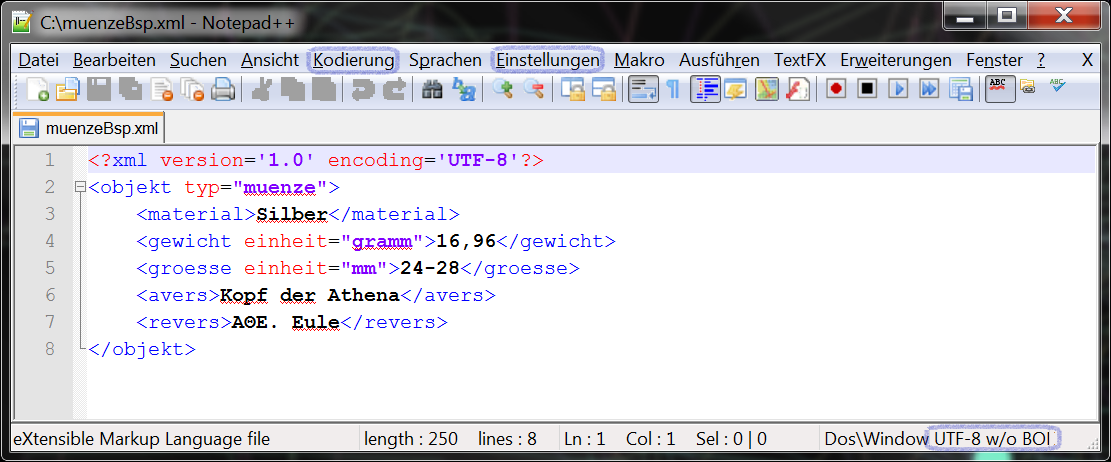
\includegraphics[width=0.99\textwidth]{bilder/text_notepadMarkierung}
  \end{center}
  \caption{Screenshot von Notepad++ mit einer geöffneten XML-Datei. Die Menüpunkte "`Einstellungen"' und "`Kodierung"' wurden hervorgehoben. Im unteren rechten Bereich ist die Anzeige der verwendeten Zeichenkodierung gekennzeichnet.}
  \label{abb:text-notepad}
\end{figure}


In \emph{TextWrangler} ist diese Option unter "`TextWrangler > Preferences > Text Encoding"' zu finden. Auch hier werden die Einstellungen der Zeichenkodierung einer vorhandenen Datei beibehalten. Zusätzlich besteht die Möglichkeit die Zeichenkodierung zu ändern, indem eine Datei über "`File > Reopen Using Encoding"' und der gewünschten Kodierung geöffnet wird. 

\begin{figure}[htb!]
  \begin{center}
    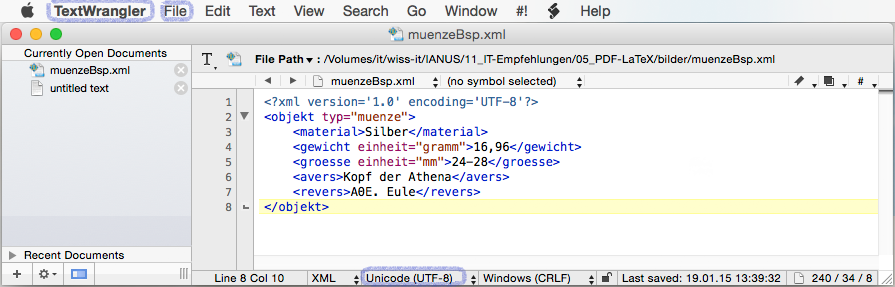
\includegraphics[width=0.99\textwidth]{bilder/text_wranglerMarkierung}
  \end{center}
  \caption{Screenshot von TextWrangler mit einer geöffneten XML-Datei. Die Menüpunkte "`TextWrangler"' und "`File"' wurden hervorgehoben. Im unteren linken Bereich ist die Anzeige der verwendeten Zeichenkodierung gekennzeichnet.}
  \label{abb:text-wrangler}
\end{figure}

%XXX? Zeilenende (Win, Unix) noch erklären?

\subparagraph{Metadaten bearbeiten und ergänzen}
In der Regel werden nur wenige Metadaten automatisch in Textdokumenten von Textverarbeitungsprogrammen wie Microsoft Word, OpenOffice Writer oder LibreOffice Writer angelegt und gespeichert. Dazu gehören vor allem technische Informationen, wie Dateigröße, Dateiname, Erstellungs- und Änderungsdatum. Auch eine Statistik mit der Anzahl der Zeichen, Wörter, Absätze etc. wird erstellt. Als Autor wird der für das jeweilige Programm angegebenen Nutzername gespeichert. Über die Menüpunkte "`Datei > Informationen > Eigenschaften"' bzw. "`Datei > Eigenschaften"' lassen sich die Angaben anpassen und ergänzen. Beispielsweise kann ein Titel, Schlagworte und ein Beschreibungstext eingefügt werden. Zusätzliche Angaben können unter "`Anpassen"' bzw. "`Benutzerdefinierte Eigenschaften"' aus einer Liste gewählt und ausgefüllt werden. Darüber hinausgehende Informationen wie beispielsweise ein Identifikator oder Angaben zur Lizenz, können in einer getrennten Text- oder XML-Datei hinterlegt werden. Ausführlichere Angaben sind in "`\href{http://www.kim-forum.org/Subsites/kim/DE/Materialien/Dokumente/dokumente_node.html\#doc42066bodyText7}{Verfahren zur Produktion interoperabler Metadaten in digitalen Dokumentenverarbeitungsprozessen}"' von Alexander Haffner (2011) zu finden.

Bei Textdokumenten bietet sich die Möglichkeit, neben einem Deckblatt auch einen Innentitel mit den relevanten Metadaten zu integrieren. Hier können zusätzlich ein Zitierhinweis und eine längere Versionshistorie untergebracht werden. Ein Beispiel für solch einen Innentitel findet sich am Anfang der PDF-Version dieser Empfehlungen.

In reinen Textdateien, wie TXT oder \emph{plain text}, können keine Metadaten als Eigenschaften in das Dateiformat integriert werden. Es besteht jedoch die Möglichkeit, sie mit in das Dokument einzutragen oder eine separate Datei anzulegen. Auszeichnungssprachen bieten zu diesem Zweck meist einen eigens dafür vorgesehenen Bereich am Beginn der Datei, den sogenannten Kopfbereich oder \emph{Header}.

Tools wie beispielsweise das \href{http://meta-extractor.sourceforge.net/}{Metadata Extraction Tool} oder eines der Tools, die auf \href{http://www.forensicswiki.org/wiki/Document_Metadata_Extraction\#Office_Files}{forensicswiki.org} gelistet sind, können verwendet werden, um Metadaten zu extrahieren und in separaten Dateien zu speichern.

\begin{flushleft}
	Metadata Extraction Tool: \urllist{http://meta-extractor.sourceforge.net/}
	Tools zur Extraktion von Metadaten: \urllist{http://www.forensicswiki.org/wiki/Document_Metadata_Extraction\#Office_Files}
\end{flushleft}



\subparagraph{Digitalisate} \label{Digitalisate-Texte} 
Für die Digitalisierung von analogen Schriftstücken mittels eines Scanners gibt es ausführliche Hinweise in den \href{http://www.dfg.de/formulare/12_151/}{\emph{DFG-Praxisregeln "Digitalisierung"}}.

Eine kurze Übersicht aus dem oben angegebenen Dokument ist in der folgenden Tabelle zu finden:

\begin{center}
	\begin{tabular}{p{0.53\textwidth} l}
		\toprule
		Größe des kleinsten signifikanten Zeichens & Auflösung \\ \midrule
		bis 1 mm & min. 400 dpi \\
		ab 1,5 mm & min. 300 dpi \\ \cmidrule(r){1-2}
		\multicolumn{2}{l}{Die Speicherung erfolgt in Form unkomprimierter Baseline TIFF-Dateien.} \\
		\bottomrule    
	\end{tabular}
\end{center}

Um zu verdeutlichen, dass von der Vorlage nichts abgeschnitten wurde, sollten Seiten immer vollständig mit einem umlaufenden Rand gesichert werden.

Der Scan eines Textdokumentes ist zunächst eine digitale Rastergrafik, die erst durch optische Zeichenerkennung (OCR, von engl. \emph{Optical Character Recognition}) oder Transkription zu einem digitalen Textdokument wird. Mit OCR bearbeitete Texte benötigen eine Angabe zur Genauigkeit der Buchstaben in Prozent. Ab Seite 30 der Praxisregeln wird die Ermittlung der Buchstabengenauigkeit beschrieben.

Die DFG-Praxisregeln beziehen sich teilweise auf die Richtlinien der Federal Agencies Digitization Guidelines Initiative (FADGI), die in englischer Sprache in dem Dokument "`\href{http://www.digitizationguidelines.gov/guidelines/FADGI_Still_Image-Tech_Guidelines_2010-08-24.pdf}{\emph{Technical Guidelines for Digitizing Cultural Heritage Materials: Creation of Raster Image Master Files}}"' zu finden sind.

Bei der Neubeschaffung eines Scanners muss darauf geachtet werden, dass er die Mindestanforderungen für den jeweiligen Digitalisierungszweck erfüllt.


\paragraph{Quellen}
\begin{flushleft}
%1. Autor -- 2. Autor, Titel (Jahr) \urllist{}\\
Archaeology Data Service, Documents and Digital Texts: A Guide to Good Practice \urllist{http://guides.archaeologydataservice.ac.uk/g2gp/TextDocs_Toc}
A. Haffner, Verfahren zur Produktion interoperabler Metadaten in digitalen Dokumentenverarbeitungsprozessen (Frankfurt am Main 2011) \urllist{http://www.kim-forum.org/Subsites/kim/DE/Materialien/Dokumente/dokumente_node.html\#doc42066bodyText7}
R. Ishida, Zeichencodierung für Anfänger \urllist{http://www.w3.org/International/questions/qa-what-is-encoding}
R. Ishida, Zeichencodierungen: grundlegende Konzepte \urllist{http://www.w3.org/International/articles/definitions-characters/}
A. Morrison -- M. Popham -- K. Wikander, Creating and Documenting Electronic Texts: A Guide to Good Practice \urllist{http://ota.ahds.ac.uk/documents/creating/cdet/index.html} %XXX Jahr? ISSN: 1463-5194
A. Morrison -- M. Wynne, AHDS Preservation Handbook: Marked-up Textual Data (2005) \urllist{http://ota.ahds.ac.uk/documents/preservation/preservation_markup.pdf}
nestor (Hrsg.) Nicht von Dauer: Kleiner Ratgeber für die Bewahrung digitaler Daten in Museen (2009) 22-28 \abstand
H. Neuroth -- A. Oßwald -- R. Scheffel -- S. Strathmann -- M. Jehn (Hrsg.) nestor Handbuch. Eine kleine Enzyklopädie der digitalen Langzeitarchiverung. Version 2.0 (2009) Kap. 17.2 \abstand
G. Rehm, Texttechnologische Grundlagen, in: K.-U. Carstensen -- Ch. Ebert -- C. Endriss -- S. Jekat -- R. Klabunde -- H. Langer (Hrsg.) Computerlinguistik und Sprachtechnologie. Eine Einführung $^2$(München 2004) 138-147 \abstand
TEI (Hrsg.) A Gentle Introduction to XML \urllist{http://www.tei-c.org/release/doc/tei-p5-doc/de/html/SG.html}
DFG-Praxisregeln "`Digitalisierung"' \urllist{http://www.dfg.de/formulare/12_151/12_151_de.pdf}
FAQ zu UTF und BOM \urllist{http://www.unicode.org/faq/utf_bom.html}

\quelltyp{Formatspezifikationen}
ODT: \urllist{https://www.oasis-open.org/standards\#opendocumentv1.2}
DOCX: ECMA-376 \urllist{http://www.ecma-international.org/publications/standards/Ecma-376.htm}
SGML: ISO 8879 \urllist{http://www.iso.org/iso/catalogue_detail.htm?csnumber=16387}
HTML: WHATWG -- W3C (Hrsg.) HTML5 (2014) \urllist{http://www.w3.org/TR/html5/}
XML: T. Bray -- J. Paoli -- C. M. Sperberg-McQueen -- E. Maler, F. Yergeau, Extensible Markup Language (XML) 1.0 $^5$(2008) \urllist{http://www.w3.org/TR/xml/}
XSD: \urllist{http://www.w3.org/TR/\#tr_XML_Schema}
TEI: Text Encoding Initiative (TEI) \urllist{http://www.tei-c.org/index.xml}
TEI: TEI (Hrsg.) P5: Richtlinien für die Auszeichnung und den Austausch elektronischer Texte \urllist{http://www.tei-c.org/release/doc/tei-p5-doc/de/html/index.html}
Unicode: Unicode Consortium (Hrsg.) Unicode 7.0.0 \urllist{http://www.unicode.org/versions/Unicode7.0.0/}

\quelltyp{Tools und Programme}
Metadata Extraction Tool: \urllist{http://meta-extractor.sourceforge.net/}
Tools zur Extraktion von Metadaten: \urllist{http://www.forensicswiki.org/wiki/Document_Metadata_Extraction\#Office_Files}
Notepad++: \urllist{http://www.notepad-plus-plus.org/}
TextWrangler: \urllist{http://www.barebones.com/products/textwrangler/}
Vergleich von Texteditoren auf Wikipedia: \urllist{http://en.wikipedia.org/wiki/Comparison_of_text_editors}
\end{flushleft}